% UML diagram tried: jednotný informačný model profilu AI modelu.
% Samostatne: latexmk -pdf profil.tex   V dokumentácii: \includestandalone{uml/profil}
\documentclass[tikz,border=4pt]{standalone}
\usepackage[T1]{fontenc}
\usepackage{lmodern}
\usepackage{amssymb}
\usetikzlibrary{arrows.meta,shapes.multipart}
\begin{document}
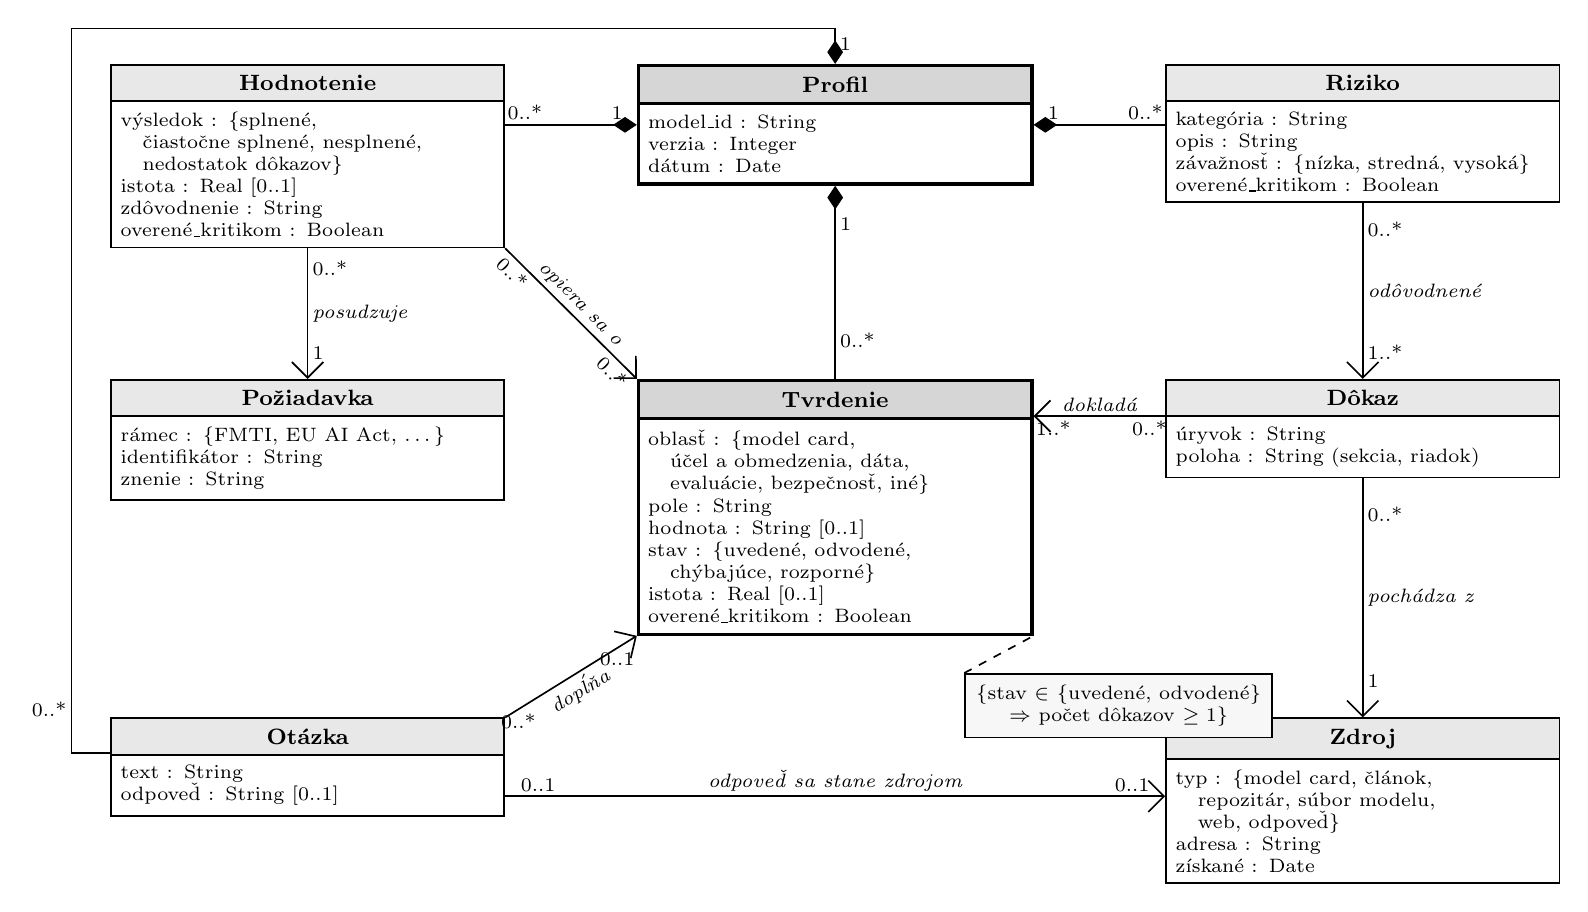
\begin{tikzpicture}[
    font=\footnotesize,
    trieda/.style={draw, semithick, rectangle split, rectangle split parts=2,
        rectangle split part fill={gray!18, white},
        text width=4.75cm, anchor=north, inner sep=3.5pt, font=\scriptsize},
    hlavna/.style={trieda, very thick, rectangle split part fill={gray!32, white}},
    poznamka/.style={draw, semithick, fill=gray!6, font=\scriptsize, align=center, inner sep=4pt},
    kompozicia/.style={{Diamond[length=3mm, width=2mm]}-, semithick},
    asoc/.style={-{Straight Barb[length=2mm]}, semithick},
    nas/.style={font=\scriptsize, inner sep=1.5pt},
    rola/.style={font=\scriptsize\itshape, inner sep=1.5pt}
]
\newcommand\meno[1]{\centerline{\textbf{\footnotesize #1}}}
\newcommand\odsad{\\\hspace*{1em}}

    %%% triedy
    \node[trieda] (hodn) at (0,0) {\meno{Hodnotenie}
        \nodepart{second}výsledok : \{splnené,\odsad čiastočne splnené, nesplnené,\odsad nedostatok dôkazov\}\\istota : Real [0..1]\\zdôvodnenie : String\\overené\_kritikom : Boolean};
    \node[hlavna] (profil) at (6.7,0) {\meno{Profil}
        \nodepart{second}model\_id : String\\verzia : Integer\\dátum : Date};
    \node[trieda] (riziko) at (13.4,0) {\meno{Riziko}
        \nodepart{second}kategória : String\\opis : String\\závažnosť : \{nízka, stredná, vysoká\}\\overené\_kritikom : Boolean};

    \node[trieda] (poz) at (0,-4.0) {\meno{Požiadavka}
        \nodepart{second}rámec : \{FMTI, EU AI Act, \ldots\}\\identifikátor : String\\znenie : String};
    \node[hlavna] (tvrd) at (6.7,-4.0) {\meno{Tvrdenie}
        \nodepart{second}oblasť : \{model card,\odsad účel a~obmedzenia, dáta,\odsad evaluácie, bezpečnosť, iné\}\\pole : String\\hodnota : String [0..1]\\stav : \{uvedené, odvodené,\odsad chýbajúce, rozporné\}\\istota : Real [0..1]\\overené\_kritikom : Boolean};
    \node[trieda] (dokaz) at (13.4,-4.0) {\meno{Dôkaz}
        \nodepart{second}úryvok : String\\poloha : String (sekcia, riadok)};

    \node[trieda] (otazka) at (0,-8.3) {\meno{Otázka}
        \nodepart{second}text : String\\odpoveď : String [0..1]};
    \node[trieda] (zdroj) at (13.4,-8.3) {\meno{Zdroj}
        \nodepart{second}typ : \{model card, článok,\odsad repozitár, súbor modelu,\odsad web, odpoveď\}\\adresa : String\\získané : Date};

    %%% obmedzenie: hlavný princíp „žiadne zistenie bez dôkazu“
    \node[poznamka] (ob) at (10.3,-8.15) {\{stav $\in$ \{uvedené, odvodené\}\\$\Rightarrow$ počet dôkazov $\geq 1$\}};
    \draw[dashed, semithick] (ob.north west) -- (tvrd.south east);

    %%% kompozície: profil vlastní svoje časti
    \draw[kompozicia] (profil.west) -- node[nas, above, pos=0.15] {1} node[nas, above, pos=0.85] {0..*} (hodn.east |- profil.west);
    \draw[kompozicia] (profil.east) -- node[nas, above, pos=0.15] {1} node[nas, above, pos=0.85] {0..*} (riziko.west |- profil.east);
    \draw[kompozicia] (profil.south) -- node[nas, right, pos=0.2] {1} node[nas, right, pos=0.8] {0..*} (tvrd.north);
    \draw[kompozicia] (profil.north) -- ++(0,0.45) -| node[nas, left, pos=0.97] {0..*} (-3.0,-8.75) -- (otazka.west |- 0,-8.75);
    \node[nas, right] at ([yshift=0.25cm]profil.north) {1};

    %%% asociácie
    \draw[asoc] (dokaz.west |- dokaz.text split) -- node[rola, above] {dokladá} node[nas, below, pos=0.12] {0..*} node[nas, below, pos=0.85] {1..*} (tvrd.east |- dokaz.text split);
    \draw[asoc] (dokaz.south) -- node[rola, right] {pochádza z} node[nas, right, pos=0.15] {0..*} node[nas, right, pos=0.85] {1} (zdroj.north);
    \draw[asoc] (riziko.south) -- node[rola, right] {odôvodnené} node[nas, right, pos=0.15] {0..*} node[nas, right, pos=0.85] {1..*} (dokaz.north);
    \draw[asoc] (hodn.south east) -- node[rola, above, sloped] {opiera sa o} node[nas, below, sloped, pos=0.12] {0..*} node[nas, below, sloped, pos=0.88] {0..*} (tvrd.north west);
    \draw[asoc] (hodn.south) -- node[rola, right] {posudzuje} node[nas, right, pos=0.15] {0..*} node[nas, right, pos=0.8] {1} (poz.north);
    \draw[asoc] (otazka.north east) -- node[rola, below, sloped] {dopĺňa} node[nas, below, pos=0.1] {0..*} node[nas, below, pos=0.85] {0..1} (tvrd.south west);
    \draw[asoc] (otazka.east |- 0,-9.3) -- node[rola, above, pos=0.5] {odpoveď sa stane zdrojom} node[nas, above, pos=0.05] {0..1} node[nas, above, pos=0.95] {0..1} (zdroj.west |- 0,-9.3);
\end{tikzpicture}
\end{document}
